% Self-adaptive (WamOL) loss-weight mechanism used in the DCPINN calibration
% loop (notebooks/PINN_implementation.ipynb, calibration()/update_loss_weights()).
%
% Solid arrows  = the main training loop, run every epoch.
% Dashed arrows = the self-adaptive weight update, run every 100 epochs
%                 (config.balancing, DCPINN only).
\documentclass[tikz, border=10pt]{standalone}
\usepackage{tikz}
\usepackage{amsmath, amssymb}
\usetikzlibrary{arrows.meta, positioning, fit, backgrounds}

% ---------------------------------------------------------------------------
% Spacing macros -- adjust here, not per-node, to keep the layout consistent.
% ---------------------------------------------------------------------------
\def\vsep{1.3cm}   % vertical distance between main-loop stages
\def\hsep{0.9cm}   % horizontal gap between the three loss branches
\def\sidesep{3.0cm}% horizontal offset of the adaptive-weight subsystem

% Greyscale palette; a single muted fill tints the adaptive subsystem so it
% reads as a distinct region without relying on colour alone (it is already
% distinguished by the dashed border and by its dashed connections).
\definecolor{subsysfill}{RGB}{240,240,240}

\begin{document}
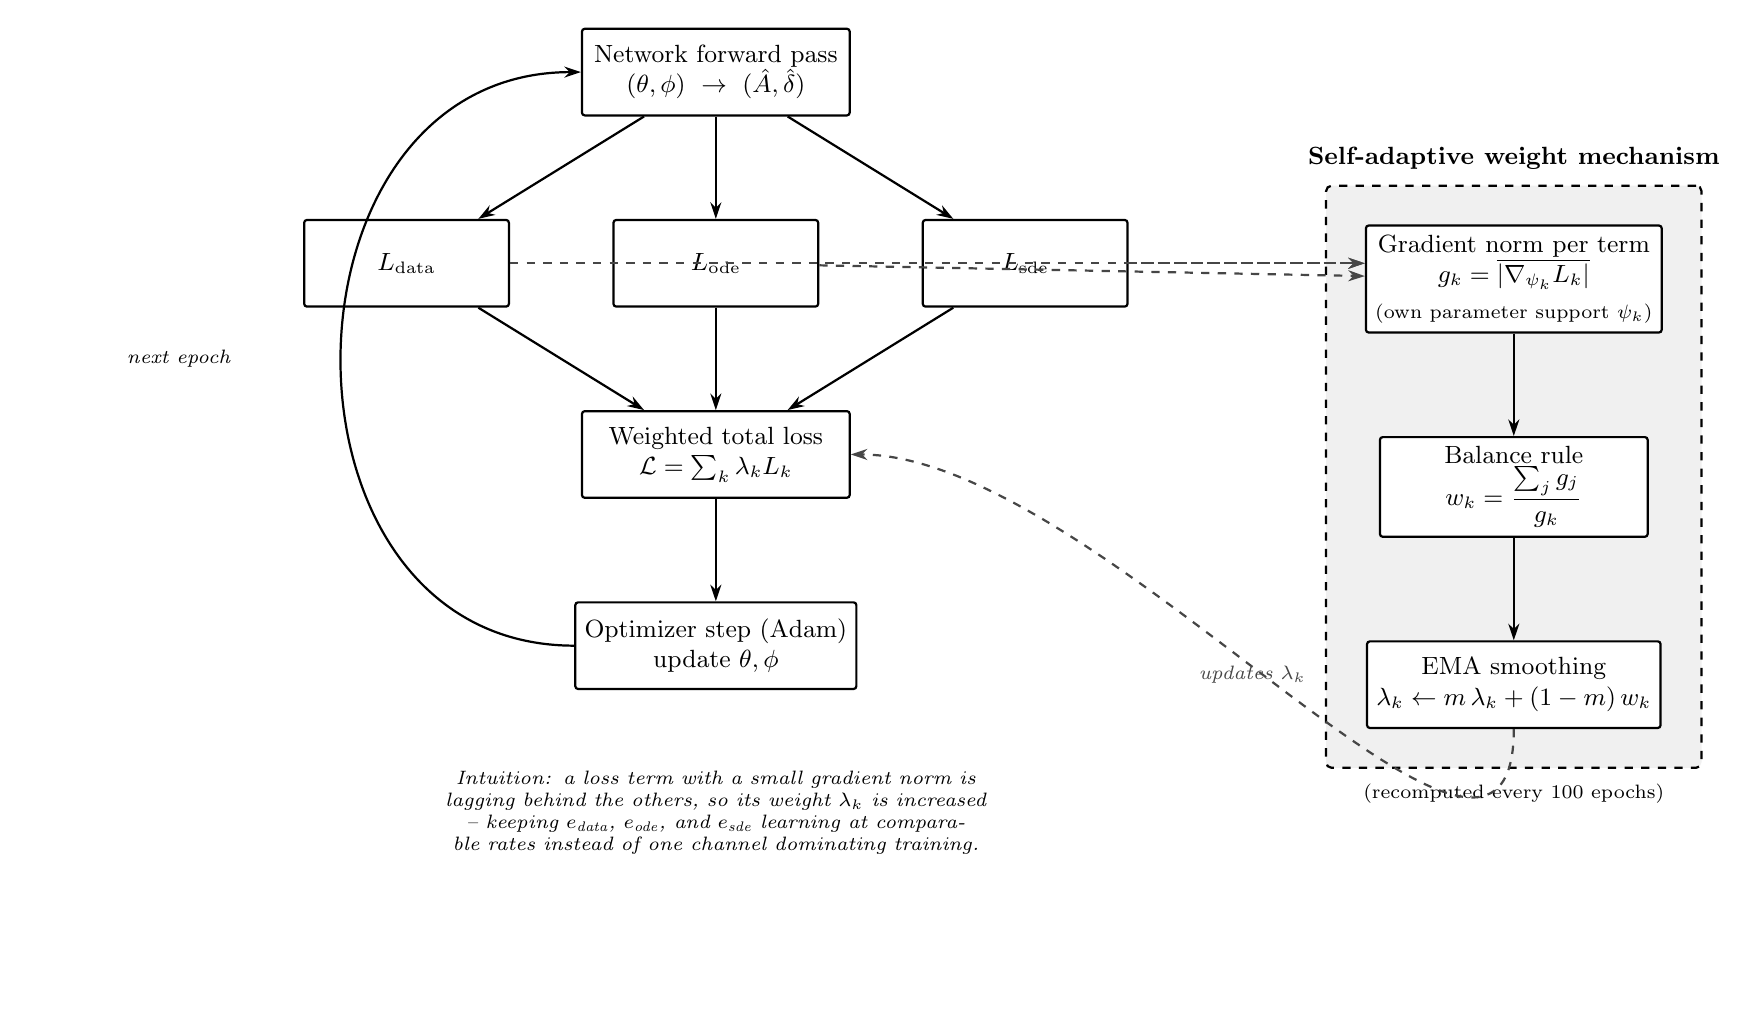
\begin{tikzpicture}[>=Stealth]

  \tikzset{
    block/.style = {
      rectangle, draw, thick, rounded corners=1pt,
      minimum width=3.4cm, minimum height=1.1cm,
      align=center, font=\small, fill=white
    },
    lossblock/.style = {
      block, minimum width=2.6cm
    },
    subsysbox/.style = {
      rectangle, draw, thick, dashed, rounded corners=2pt,
      fill=subsysfill, inner sep=14pt
    },
    mainflow/.style = {
      -{Stealth[length=6pt, width=4pt]}, thick, solid
    },
    adaptiveflow/.style = {
      -{Stealth[length=6pt, width=4pt]}, thick, dashed, gray!55!black
    },
    lbl/.style = {
      font=\scriptsize\itshape, align=center, text width=3.6cm
    }
  }

  % --- Main loop: run every epoch -------------------------------------------
  \node (fwd)   [block] {Network forward pass\\ $(\theta,\phi)\ \to\ (\hat{A},\hat{\delta})$};

  \node (ldata) [lossblock, below left=\vsep and \hsep of fwd]  {$L_{\text{data}}$};
  \node (lode)  [lossblock, below=\vsep of fwd]                {$L_{\text{ode}}$};
  \node (lsde)  [lossblock, below right=\vsep and \hsep of fwd] {$L_{\text{sde}}$};

  \node (wsum)  [block, below=\vsep of lode]
    {Weighted total loss\\ $\mathcal{L} = \sum_k \lambda_k L_k$};

  \node (opt)   [block, below=\vsep of wsum]
    {Optimizer step (Adam)\\ update $\theta,\phi$};

  % --- Self-adaptive weight subsystem: run every 100 epochs -----------------
  \node (gnorm) [block, right=\sidesep of lsde, yshift=-0.2cm]
    {Gradient norm per term\\ $g_k = \overline{\left|\nabla_{\psi_k} L_k\right|}$\\[2pt]
     {\scriptsize (own parameter support $\psi_k$)}};

  \node (brule) [block, below=\vsep of gnorm]
    {Balance rule\\ $w_k = \dfrac{\sum_j g_j}{g_k}$};

  \node (ema)   [block, below=\vsep of brule]
    {EMA smoothing\\ $\lambda_k \leftarrow m\,\lambda_k + (1-m)\,w_k$};

  \begin{scope}[on background layer]
    \node (subsys) [subsysbox, fit=(gnorm)(brule)(ema)] {};
  \end{scope}
  \node [font=\small\bfseries, above=2pt of subsys.north]
    {Self-adaptive weight mechanism};
  \node [font=\scriptsize, below=2pt of subsys.south]
    {(recomputed every 100 epochs)};

  % --- Main loop edges (solid, every epoch) ---------------------------------
  \draw [mainflow] (fwd)   -- (ldata);
  \draw [mainflow] (fwd)   -- (lode);
  \draw [mainflow] (fwd)   -- (lsde);
  \draw [mainflow] (ldata) -- (wsum);
  \draw [mainflow] (lode)  -- (wsum);
  \draw [mainflow] (lsde)  -- (wsum);
  \draw [mainflow] (wsum)  -- (opt);

  % Loop-back: optimizer step feeds the next forward pass.
  \draw [mainflow]
    (opt.west) to [out=180, in=180, looseness=1.4]
    node [lbl, left=2pt, midway, xshift=-2pt] {next epoch}
    (fwd.west);

  % --- Adaptive subsystem edges (dashed, every 100 epochs) ------------------
  \draw [adaptiveflow] (ldata) -- (gnorm.west |- ldata);
  \draw [adaptiveflow] (lode)  -- (gnorm);
  \draw [adaptiveflow] (lsde)  -- (gnorm.west |- lsde);
  \draw [mainflow]     (gnorm) -- (brule);
  \draw [mainflow]     (brule) -- (ema);
  \draw [adaptiveflow]
    (ema.south) to [out=-90, in=0, looseness=0.9]
    node [lbl, below, pos=0.55, xshift=6pt] {updates $\lambda_k$}
    (wsum.east);

  % --- Intuition note --------------------------------------------------------
  \node [lbl, text width=8.5cm, font=\scriptsize\itshape,
         below=0.9cm of opt, align=center]
    {Intuition: a loss term with a small gradient norm is lagging behind the
     others, so its weight $\lambda_k$ is increased -- keeping $e_{\text{data}}$,
     $e_{\text{ode}}$, and $e_{\text{sde}}$ learning at comparable rates instead
     of one channel dominating training.};

\end{tikzpicture}
\end{document}
